\section{Luồng chat stream có phân nhánh Rasa/RAG và fallback RAG}

Luồng này mô tả trường hợp hệ thống hỗ trợ trả lời theo chế độ stream, đồng thời có thể phân nhánh giữa xử lý bằng Rasa và xử lý bằng RAG. Đây là luồng quan trọng nhất đối với các câu hỏi tự nhiên, vì nó cho thấy cách hệ thống kết hợp rule-based dialogue với truy xuất tri thức từ kho tài liệu.

\begin{figure}[H]
    \centering
    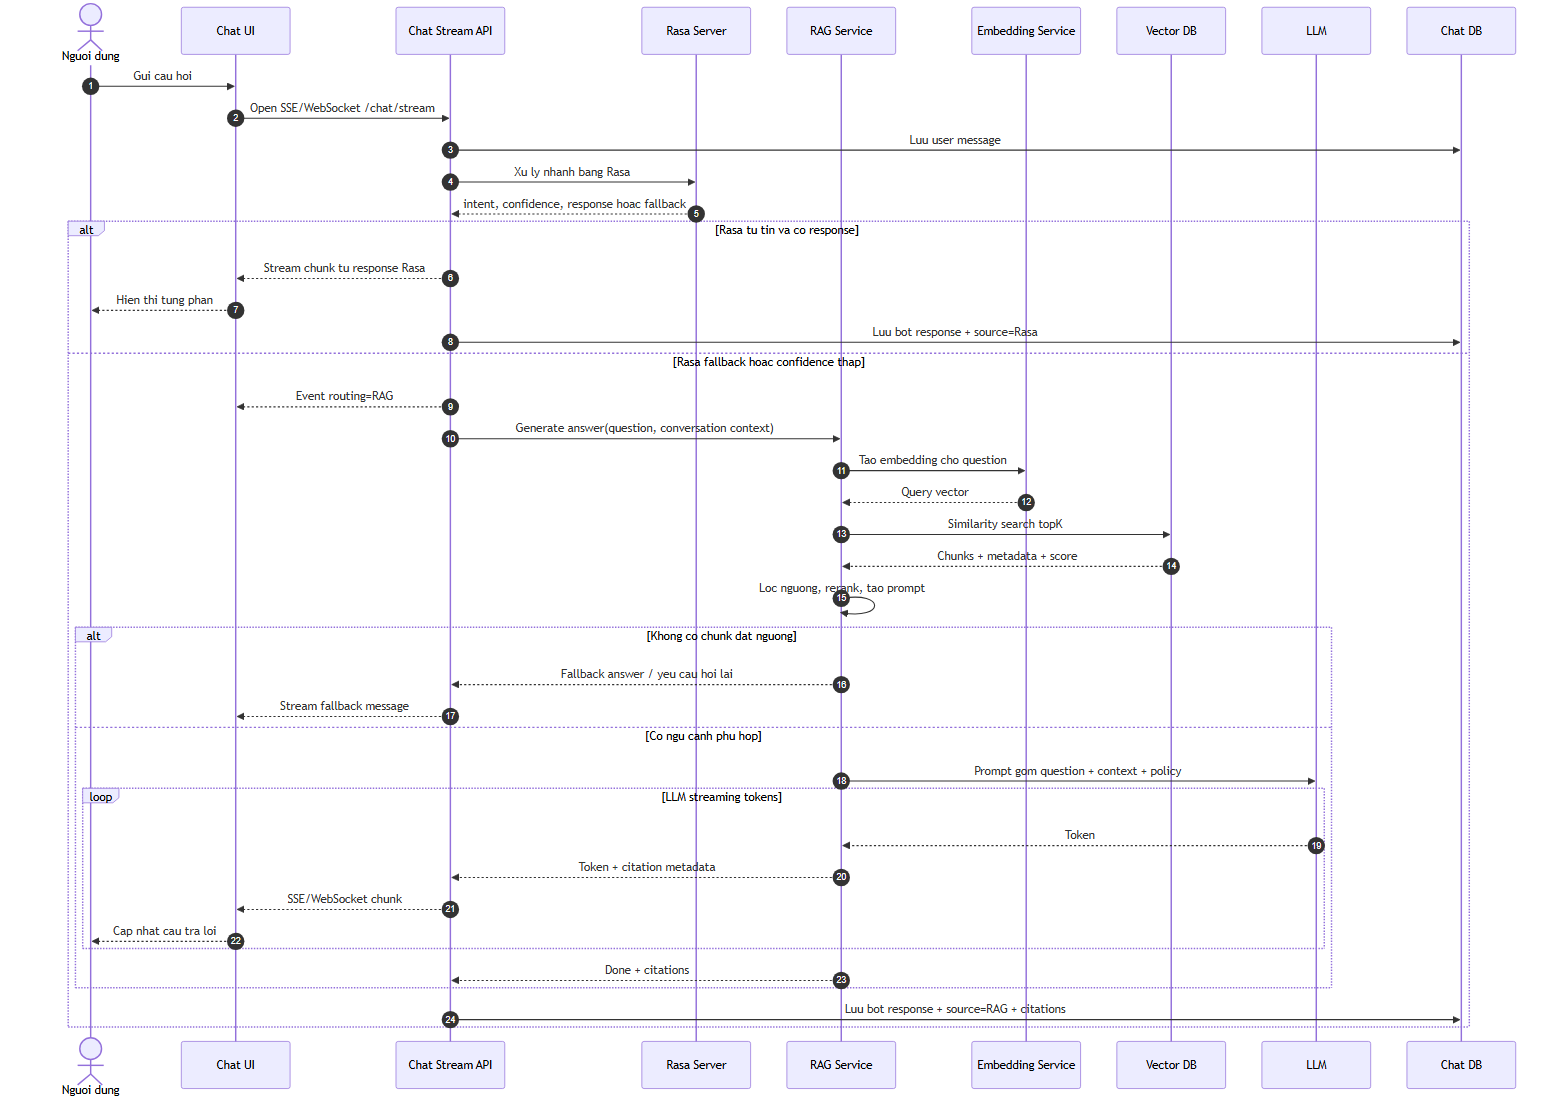
\includegraphics[width=\textwidth]{content/source/mermaid_sequence/seq_02.png}
    \caption{Luồng chat stream có phân nhánh Rasa/RAG và fallback RAG}
\end{figure}

Ở pha đầu, người dùng gửi câu hỏi và frontend mở kết nối nhận phản hồi theo dòng. Flask API đóng vai trò điều phối: nếu intent trong Rasa đủ tin cậy thì phản hồi đi theo nhánh hội thoại thông thường; nếu rơi vào \path{nlu_fallback}, action của Rasa sẽ gọi sang KmaRAG để truy xuất ngữ cảnh, dựng prompt và sinh câu trả lời. Nhờ cơ chế stream, câu trả lời có thể được đẩy dần về giao diện thay vì chờ hoàn tất toàn bộ. Kiến trúc này giữ được tốc độ xử lý cho câu hỏi phổ biến, đồng thời vẫn hỗ trợ câu hỏi dài hoặc phụ thuộc vào tài liệu.
